% !TEX root = ../main.tex
\pagebreak[0]
\section{\emph{Global} component}\label{sec:global-component}

\begin{figure}[htbp]
\centering
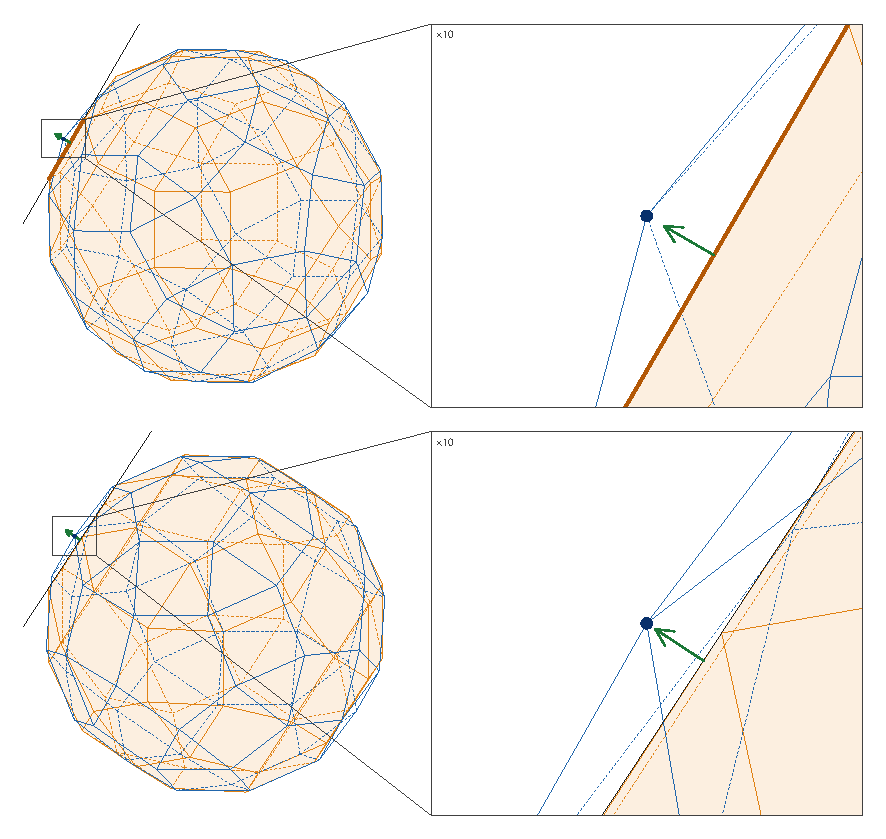
\includegraphics[width=\linewidth]{figures/global}
\caption{Two poke configurations eliminated by the Global component, at the midpoints of two search boxes of the final certificate: $[7/48,7/80,(1/20,-1/20,1/4)]$ and $[3/16,23/80,(-1/40,-13/40,-1/8)]$. Left: the projected edges of \fc{Hole}{the hole (orange)} and of \fc{Plug}{the plug (blue)}, dashed on each body's far side, with \fc{Hole}{the hole's shadow lightly tinted}. Right: the marked windows, enlarged ten times. Black: the supporting line of the hole's shadow for the direction of the hole edge named in the box's record; \fc{Support}{thick brown: the part of the hole's silhouette on that line} (on the right, a single vertex attains it); \fc{Normal}{green: the outward normal}, drawn from the foot of the perpendicular from \fc{Vertex}{the record's plug vertex (dark blue dot)}, which lies strictly beyond the line. The component certifies this separation at every configuration of the box.}
\label{fig:global-examples}
\end{figure}

A projected plug vertex protruding beyond the hole's shadow prevents a fit.
The \emph{Global} component certifies that such protrusion persists
throughout a box. This geometric idea
also underlies the global theorem of
\citet[Section~4, Theorem~17]{SteiningerYurkevichNopertV2}.

\subsection{Eliminating \emph{poke} configurations}\label{subsec:eliminating-poke-configurations}

Fix a poke configuration. At least one projected plug vertex lies outside
the hole's shadow: otherwise convexity would put the entire plug shadow
inside it. We use the orthogonal screen for the separation picture.
There is a direction along which that vertex extends further
than every point of the hole's shadow. To see the comparison, project the
two shadows onto a line parallel to this direction. The selected plug
vertex lies beyond the interval occupied by the hole shadow.

For a nonzero vector $\mathbf n$ in the orthogonal screen plane, the largest
value of $\mathbf n\cdot\mathbf h$ over points $\mathbf h$ of the hole shadow
is its \emph{support value}
in that direction. The line where this value is attained is a
\emph{supporting line}: the whole shadow lies on one side of it.
We call $\mathbf n$ a \emph{support direction}. Since
$\mathbf n\cdot\mathbf u=0$, taking a dot product with $\mathbf n$ gives
the same value before and after projection. Thus a selected plug vertex
$\mathbf v_p\in V$ is separated from the hole shadow if
\begin{equation}\label{eq:point-support-separation}
  \mathbf n\cdot R_P(\mathbf r)\mathbf v_p
     >\max_{\mathbf v\in V}\mathbf n\cdot\mathbf v.
\end{equation}
Due to convexity and the linearity of the dot product, the maximum over
vertices is also the maximum over their convex hull.

\paragraph{Stability of the margin.}
A sufficiently small change of configuration preserves a strict
separation. Before deriving the inequalities used to check a whole box,
we quantify this stability in terms of the margin introduced in
\cref{subsec:the-margin-function-and-fit-poke-touch}.

\begin{lemma}[Lipschitz bound for the margin]\label{lem:lipschitz-bound-for-the-margin}
  For configurations $c,c'\in B_0$,
  \begin{equation}\label{eq:margin-lipschitz-bound}
    |M_{\mathcal R}(c)-M_{\mathcal R}(c')|
       \le16\lVert c-c'\rVert,
  \end{equation}
  where the distance is Euclidean distance between the five parameters,
  as in \cref{subsec:component-hierarchy}.
\end{lemma}
\begin{proof}
  First, $\mathcal R$ contains the ball of radius two about zero and lies
  in the ball of radius five. For the inner bound, average the three cyclic
  permutations of $(1,1,\varphi^3)$, applying the same coordinate sign
  choices to each. This places all eight corners of the cube with half-side
  $(4+\sqrt5)/3>2$ inside $\mathcal R$. For the outer bound, all vertices
  whose coordinates are given in \cref{eq:rhombicosidodecahedron-vertices}
  have distance $\sqrt{11+4\sqrt5}<5$ from the origin. Orthogonal shadows
  therefore give $M_{\mathcal R}(c)\le5/2$ for every configuration.
  The same bound holds in rational screen coordinates: applying the same
  invertible linear map to both shadows preserves scaled containment and
  hence the margin, by \cref{lem:margin-and-containment}.

  \paragraph{Rotation and shadow displacement.}
  We use the Euclidean operator norm for matrices,
  $\lVert A\rVert=\max_{\lVert\mathbf v\rVert=1}\lVert A\mathbf v\rVert$.
  Put $\delta_{s,t}=\lVert(s,t)-(s',t')\rVert$ and
  $\delta_{\mathbf r}=\lVert\mathbf r-\mathbf r'\rVert$. To bound the motion
  of the shadow vertices, we use
  \begin{equation}\label{eq:rotation-and-screen-displacement-bounds}
    \begin{aligned}
      \lVert R_P(\mathbf r)-R_P(\mathbf r')\rVert&\le2\delta_{\mathbf r},\\
      \lVert L_{s,t}-L_{s',t'}\rVert&=\delta_{s,t},\\
      \lVert L_{s,t}\rVert&\le\frac43.
    \end{aligned}
  \end{equation}
  These estimates follow from the rotation and screen formulas
  \cref{eq:relative-rotation,eq:screen-map} and the ranges defining $B_0$.
  For the rotation estimate, write
  ${[\mathbf r]}_\times\mathbf v=\mathbf r\times\mathbf v$. The vector
  triple-product identity gives
  ${[\mathbf r]}_\times^2=\mathbf r\mathbf r^{\mathsf T}-\lVert\mathbf r\rVert^2I$,
  and ${[\mathbf r]}_\times\mathbf r=\mathbf0$. Multiplying by $I-{[\mathbf r]}_\times$
  therefore verifies the inverse formula
  \[
    {(I-{[\mathbf r]}_\times)}^{-1}
      =\frac{I+{[\mathbf r]}_\times+\mathbf r\mathbf r^{\mathsf T}}
             {1+\lVert\mathbf r\rVert^2}.
  \]
  The rotation formula \cref{eq:relative-rotation} can therefore be written as
  \[
    R_P(\mathbf r)=2{(I-{[\mathbf r]}_\times)}^{-1}-I.
  \]
  Also, orthogonality of a cross product to its factors gives
  \[
    \lVert(I-{[\mathbf r]}_\times)\mathbf v\rVert^2
      =\lVert\mathbf v\rVert^2+\lVert {[\mathbf r]}_\times\mathbf v\rVert^2,
  \]
  so this inverse has operator norm at most one. Apply the inverse-difference
  identity $A^{-1}-B^{-1}=A^{-1}(B-A)B^{-1}$ to
  $A=I-{[\mathbf r]}_\times$ and $B=I-{[\mathbf r']}_\times$. Since
  $\lVert\mathbf a\times\mathbf v\rVert\le\lVert\mathbf a\rVert\lVert\mathbf v\rVert$,
  we obtain
  \[
    \lVert R_P(\mathbf r)-R_P(\mathbf r')\rVert
      \le2\lVert {[\mathbf r]}_\times-{[\mathbf r']}_\times\rVert
      \le2\lVert\mathbf r-\mathbf r'\rVert=2\delta_{\mathbf r}.
  \]

  By \cref{eq:screen-map}, the difference $L_{s,t}-L_{s',t'}$ sends
  $\mathbf v$ to $(-(s-s')v_3,-(t-t')v_3)$, so its operator norm is
  $\delta_{s,t}$. Moreover,
  \[
    L_{s,t}L_{s,t}^{\mathsf T}
      =\begin{pmatrix}1+s^2&st\\st&1+t^2\end{pmatrix}
  \]
  has eigenvalues $1$ and $1+s^2+t^2$. The ranges $0\le s\le2/3$ and
  $0\le t\le2/5$ in \cref{eq:search-rectangle} therefore give
  \[
    \lVert L_{s,t}\rVert=\sqrt{1+s^2+t^2}
      \le\sqrt{1+\frac49+\frac4{25}}=\frac{19}{15}<\frac43.
  \]
  Using the vertex bound above, set
  $\delta_H=5\delta_{s,t}$ and
  $\delta_P=5\delta_{s,t}+(40/3)\delta_{\mathbf r}$.
  Corresponding hole vertices satisfy
  \[
    \lVert L_{s,t}\mathbf v-L_{s',t'}\mathbf v\rVert
      \le5\delta_{s,t}=\delta_H.
  \]
  For plug vertices, write the difference as
  \[
    (L_{s,t}-L_{s',t'})R_P(\mathbf r)\mathbf v
      +L_{s',t'}\bigl(R_P(\mathbf r)-R_P(\mathbf r')\bigr)\mathbf v.
  \]
  Rotations preserve length, so the estimates just proved bound its norm by
  \[
    5\delta_{s,t}+\frac43\cdot2\delta_{\mathbf r}\cdot5
      =5\delta_{s,t}+\frac{40}{3}\delta_{\mathbf r}=\delta_P.
  \]
  Taking convex combinations
  of corresponding vertices with the same coefficients gives the same bounds
  for points of the filled shadows, in both directions. Each rational-screen shadow
  contains the radius-two disk, since the spatial body contains the
  radius-two ball and $L_{s,t}(v_1,v_2,0)=(v_1,v_2)$.

  \paragraph{From displacement to margin.}
  Let $m=M_{\mathcal R}(c)$ be the margin at $c$. Each point
  $\mathbf p'\in P_{c'}$ of the plug shadow at $c'$ is within
  $\delta_P$ of some $\mathbf p\in P_c$. Since $P_c\subseteq mH_c$,
  write $\mathbf p=m\mathbf h$ for a point $\mathbf h\in H_c$ of the
  hole shadow at $c$. Choose $\mathbf h'\in H_{c'}$ within
  $\delta_H$ of $\mathbf h$. Then
  \[
    \lVert\mathbf p'-m\mathbf h'\rVert\le m\delta_H+\delta_P.
  \]
  The radius-two disk and convexity of $H_{c'}$ imply
  \[
    P_{c'}\subseteq
    \left(m+\frac{m\delta_H+\delta_P}{2}\right)H_{c'}.
  \]
  Indeed, dividing
  $\mathbf p'=m\mathbf h'+(\mathbf p'-m\mathbf h')$ by the scale factor
  $m+(m\delta_H+\delta_P)/2$ gives a convex combination of
  $\mathbf h'$ and a point in the radius-two disk.
  Apply \cref{lem:margin-and-containment}, use $m\le5/2$, and interchange
  $c,c'$ to obtain
  \begin{equation}\label{eq:margin-from-shadow-displacement}
    |M_{\mathcal R}(c)-M_{\mathcal R}(c')|
      \le\frac{(5/2)\delta_H+\delta_P}{2}
      \le16\lVert c-c'\rVert.
  \end{equation}
  For the exact derivation of the last inequality, substitute the
  displacement bounds above:
  \[
    \frac{(5/2)\delta_H+\delta_P}{2}
      =\frac{35}{4}\delta_{s,t}+\frac{20}{3}\delta_{\mathbf r}.
  \]
  Since the parameter distance is Euclidean,
  $\lVert c-c'\rVert^2=\delta_{s,t}^2+\delta_{\mathbf r}^2$.
  Both $\delta_{s,t}$ and $\delta_{\mathbf r}$ are therefore at most
  $\lVert c-c'\rVert$, and
  \[
    \frac{35}{4}\delta_{s,t}+\frac{20}{3}\delta_{\mathbf r}
      \le\left(\frac{35}{4}+\frac{20}{3}\right)\lVert c-c'\rVert
      =\frac{185}{12}\lVert c-c'\rVert
      \le16\lVert c-c'\rVert.
  \]
\end{proof}

Consequently, if $M_{\mathcal R}(c)=1+\varepsilon$ with $\varepsilon>0$,
then every $c'\in B_0$ with $\lVert c'-c\rVert\le\varepsilon/32$ satisfies
$M_{\mathcal R}(c')\ge1+\varepsilon/2>1$. This gives an explicit neighbourhood consisting entirely of poke
configurations, including when $c$ lies on a boundary of $B_0$.
The constant is a convenient bound derived from the geometry.
The program checks specific support inequalities. We must still prove that those checks
succeed on sufficiently small boxes; we do so in
\cref{subsec:range-and-insufficiency-for-touch-configurations}.

\paragraph{Whole-box support inequalities.}
To choose a support direction that remains perpendicular to the changing
viewing vector, take two distinct hole vertices $\mathbf v_a,\mathbf v_b$
and a sign $\sigma\in\{-1,1\}$, and set
\begin{equation}\label{eq:moving-support-direction}
  \mathbf n(s,t)=\sigma\,\mathbf u\times(\mathbf v_b-\mathbf v_a),
  \qquad \mathbf u=(s,t,1).
\end{equation}
This vector is perpendicular to both the viewing direction and the
segment joining the projected vertices. At a fixed configuration, choosing a pair along a
silhouette edge gives a normal to its supporting line. Throughout a box,
however, the pair need not remain on the silhouette or even be an edge of
the polyhedron: the comparison with every hole vertex is what justifies the result.
If the pair projects to a single point, $\mathbf n=\mathbf0$ and no strict
separation can be certified with it.

Write $\widehat R_P(\mathbf r)=dR_P(\mathbf r)$ for the polynomial
numerator of the rotation, where $d=1+\lVert\mathbf r\rVert^2>0$
is the denominator of the rotation formula.
For each hole vertex $\mathbf v\in V$, define the \emph{gap polynomial}
\begin{equation}\label{eq:support-gap-polynomial}
  p_{\mathbf v}(c)=\mathbf n(s,t)\cdot
    \bigl(\widehat R_P(\mathbf r)\mathbf v_p-d\mathbf v\bigr).
\end{equation}
Its total degree is at most three, and its coefficients lie in
$\mathbb Q(\sqrt5)$. If
\begin{equation}\label{eq:whole-box-support-condition}
  p_{\mathbf v}(c)>0
  \qquad\text{for every }c\in B\text{ and every }\mathbf v\in V,
\end{equation}
then division by $d>0$ proves \cref{eq:point-support-separation}
at every configuration in the box. No hole vertex is singled out: the
comparison with all sixty of them is what justifies the result, so a change
inside the box in which vertices form the silhouette does not by itself
invalidate the test. The certificate record stores the plug vertex and the
ordered hole-vertex pair, whose order fixes the sign; these data determine
all the polynomials to be checked.

\paragraph{Choosing vertices and a support direction.}
Enumerating the vertex pairs from \cref{eq:rhombicosidodecahedron-vertices}
gives exactly 120 pairs at squared distance four. Since the RID has 120
edges, each of length two in the normalisation of
\cref{subsec:the-rhombicosidodecahedron}, this list contains exactly its
edges. Comparing their difference vectors up to sign gives fifteen distinct
unoriented edge vectors. One orientation of each suffices. Reversing the
sign of $\mathbf n$ and replacing the plug vertex $\mathbf v_p$ by its
antipode $-\mathbf v_p$ only permutes the sixty gap polynomials, since
\[
  -\mathbf n\cdot\bigl(\widehat R_P(\mathbf r)\mathbf v_p-d\mathbf v\bigr)
   =\mathbf n\cdot\bigl(\widehat R_P(\mathbf r)(-\mathbf v_p)-d(-\mathbf v)\bigr)
\]
and the vertex set is centrally symmetric. The component therefore
considers $15\times60=900$ candidates: one oriented edge from each class
of parallel edges, with each plug vertex.

Only one candidate is tried on each box. It is chosen in floating point,
as the candidate whose projected plug vertex lies farthest beyond the hole
shadow's extent in the direction $\mathbf n$ at the worst of the box's 32
corners, measured as a distance in the shadow plane. If no candidate lies
beyond at every corner, none is tried. This choice only decides which
exact test to run: a rounding error can make the component try a poorer
candidate and leave the box unresolved, but never eliminate a box. Choosing
at the worst corner rather than at the midpoint matters in practice, as
the midpoint favours candidates that fail near the edges of the box.

\Cref{fig:global-examples} shows two such certified separations, enlarged.

We apply the Bernstein sign test of \cref{subsec:bernstein-coefficients}
to each polynomial $-p_{\mathbf v}$. Testing the differences between plug
and hole values directly preserves cancellations that would be lost by
bounding plug and hole values separately.
Clearing the rotation denominator preserves the inequalities' direction
because $d=1+\lVert\mathbf r\rVert^2\ge1$ for every rotation parameter $\mathbf r$.
Each gap polynomial has degree at most one in $s$ and $t$ and two in each
$r_i$, so each test inspects at most $2\cdot2\cdot3^3=108$ coefficients.

\begin{proposition}[Soundness of the \emph{Global} component]\label{prop:soundness-of-the-global-component}
  Suppose that, for a plug vertex and a signed edge direction, every
  tensor Bernstein coefficient on $B$ of each of the sixty polynomials
  $-p_{\mathbf v}$ in \cref{eq:support-gap-polynomial} is strictly negative.
  Then every configuration in $B$ is a poke configuration, and the box can be eliminated.
\end{proposition}
\begin{proof}
  \Cref{lem:bernstein-sign-test} gives $p_{\mathbf v}>0$ throughout $B$ for
  every hole vertex $\mathbf v$. Dividing by the positive $d$ proves that the
  chosen projected plug vertex lies beyond every projected hole vertex in
  direction $\mathbf n(s,t)$. It therefore lies outside their convex hull, so
  $P_c\nsubseteq H_c$ and $M_{\mathcal R}(c)>1$.
\end{proof}

\subsection{Robustly detecting potential Rupertness}\label{subsec:robustly-detecting-potential-rupertness}

The same support comparisons can identify an unexpected fit during the
search. If $c\in B_0$ and $M_{\mathcal R}(c)=1-\varepsilon$ with
$\varepsilon>0$, then
\cref{lem:lipschitz-bound-for-the-margin} gives
\[
  M_{\mathcal R}(c')\le1-\frac{\varepsilon}{2}<1
  \qquad\text{whenever }c'\in B_0\text{ and }
         \lVert c'-c\rVert\le\frac{\varepsilon}{32}.
\]
This quantifies the openness of the set of fit configurations proved in
\cref{subsec:the-margin-function-and-fit-poke-touch}. Sufficiently deep search boxes
containing $c$ lie entirely in this fitting neighbourhood by
\cref{lem:search-boxes-in-neighbourhoods}, so any point
chosen inside such a box is a fit configuration. We also need an exact
test that recognises it.

\paragraph{Exact detection at a configuration.}
The candidate normals derived from RID edges in \cref{subsec:eliminating-poke-configurations}
supply that test.
Every point outside a convex polygon violates the supporting inequality of
at least one of its edges, because the polygon is the intersection of the
closed half-planes defined by these inequalities.
An edge of the hole shadow is the projection of a supporting face of
$\mathcal R$, obtained by maximizing the corresponding spatial dot product.
Here that face can be a RID edge or one of its polygonal faces.
That face contains a RID edge whose projection is a nonzero segment
parallel to the shadow edge: otherwise all of its edges would project to
points, and so would the face. Hence one of the signed directions in
\cref{eq:moving-support-direction}, using a RID edge, strictly separates
a protruding projected plug vertex.

At a fixed configuration, discard any candidate for which
$\mathbf n=\mathbf0$. A necessary and sufficient condition for fit is
\begin{equation}\label{eq:exact-point-fit-condition}
  \max_{\mathbf v\in V}\mathbf n\cdot\widehat R_P(\mathbf r)\mathbf v
     <d\max_{\mathbf v\in V}\mathbf n\cdot\mathbf v
  \qquad\text{for every remaining candidate }\mathbf n.
\end{equation}
Necessity follows because the compact plug shadow lies in the interior
of the hole shadow, giving a strict support inequality in every nonzero
direction. Conversely, the candidate family includes a normal to every
edge of the hole shadow. Since $d>0$, these strict inequalities put the
entire plug shadow on the inner side of every edge's supporting line,
and hence in the interior of the hole shadow.

Call the left side minus the right side of
\cref{eq:exact-point-fit-condition} the \emph{score} of the candidate; fit
requires every nonzero candidate's score to be negative. At a configuration with rational
parameters, all quantities in \cref{eq:exact-point-fit-condition} lie in
$\mathbb Q(\sqrt5)$. The finite maxima, zero tests and strict comparisons
can therefore be computed exactly using
\cref{subsec:exact-representation-of-field-elements-with-integers}.
The test finishes even when vertices have coincident projections or
several vertices have the same support value; equality between the two
sides of \cref{eq:exact-point-fit-condition} fails the fit condition.
In particular, checking only that no candidate has a
positive score would also accept aligned configurations, whose scores
are all zero.

\paragraph{Detection during subdivision.}
We can add this test to the procedure in
\cref{subsec:boxes-subdivision-and-elimination}: before subdividing an
unresolved box, test its midpoint and stop if it is a fit configuration.
The midpoint is rational because every interval endpoint is rational.
Any other point in the box with rational parameters could be used instead.
The sampled point need not belong to $D$: it still describes a valid
physical configuration, and the containment test applies throughout $B_0$.

\begin{proposition}[Finite detection of fit]\label{prop:finite-detection-of-fit}
  Suppose every elimination component is sound and each component call
  finishes. If the increasing-depth search uses cyclic midpoint subdivision
  and the exact point test above, without a stopping limit, then if a
  fit exists, one is detected after finitely many processed boxes.
\end{proposition}
\begin{proof}
  If a fit exists, \cref{prop:representative-coverage} supplies a fit
  representative $c_*\in D$. No sound component can eliminate a box
  containing $c_*$. Whenever such a box is subdivided, at least one of
  its closed children still contains $c_*$, even if the point lies on
  their shared boundary.

  Write $M_{\mathcal R}(c_*)=1-\varepsilon$, where $\varepsilon>0$.
  By \cref{eq:search-box-diameter-bound}, at a sufficiently large finite
  depth every box containing $c_*$ has diameter less than
  $\varepsilon/32$. Every point in such a box is then a fit configuration
  by the Lipschitz bound above, including its sampled rational point,
  which passes \cref{eq:exact-point-fit-condition}.
  There are finitely many boxes up to that depth, and each component call
  and point test finishes, so increasing-depth processing reaches this
  box and detects a fit unless it has already detected one earlier.
\end{proof}

The sufficient depth depends on the fitting margin, so this argument gives
no uniform practical runtime estimate. On a Nopert input, completion still
requires the elimination components to resolve all boxes.
For bodies without central symmetry, the corresponding search would also
need the translation parameters discussed in
\cref{subsec:projection-containment} and effective exact comparisons for
their vertex coordinates.

The current certificate generator does not run this companion test and
has a finite depth limit; the proposition describes the procedure with
the test added and continued without such a limit.

\subsection{Range and insufficiency for \emph{touch} configurations}\label{subsec:range-and-insufficiency-for-touch-configurations}

For whole-box elimination, finding a separating direction at one
configuration is only the first step: its inequalities must be certified
on the entire box. We describe the range of the component that may try
every one of its 900 candidates. The implementation tries only the
candidate proposed by its floating-point ranking; on boxes drawn uniformly
from the final search, this never lost a box that another candidate
eliminates. The final proof does not rely on either statement: it rests on
the finished certificate, checked as described in
\cref{sec:generating-and-verifying-the-certificate}.

\begin{proposition}[Range of the \emph{Global} component]\label{prop:range-of-the-global-component}
  The range of the Global component is exactly
  \[
    \{c\in B_0:\operatorname{poke}(c)\}.
  \]
\end{proposition}
\begin{proof}
  Fix a poke configuration $c_0$. The edge argument in
  \cref{subsec:robustly-detecting-potential-rupertness} gives a
  plug vertex and signed edge direction for which every gap polynomial
  is strictly positive at $c_0$. By continuity, these sixty polynomials
  remain strictly positive on a closed neighbourhood $U$ of $c_0$ in $B_0$,
  which we may take to be a box. By
  \cref{lem:convergence-of-bernstein-coefficients}, applied to each of them
  on $U$, every box contained in $U$ whose widths are small enough passes
  the test of \cref{prop:soundness-of-the-global-component} with this
  candidate. Shrink $U$ around $c_0$ so that all of its widths are that
  small. Then every search box contained in $U$ is accepted, and $U$
  contains search boxes at arbitrarily large depths by
  \cref{lem:search-boxes-in-neighbourhoods}. This is precisely the range
  condition in \cref{def:range-of-a-component}.

  Conversely, by \cref{prop:soundness-of-the-global-component}, any accepted
  box contains only poke configurations. If $c$ is a fit or touch configuration, no box
  containing it can be accepted. By \cref{lem:search-boxes-in-neighbourhoods},
  every neighbourhood of $c$ contains a search box containing $c$, including
  when $c$ lies on a subdivision boundary. Thus $c$ cannot belong to this
  component's range.
\end{proof}

Together with the compactness reasoning in
\cref{subsec:component-hierarchy}, this shows that sufficiently fine
subdivision handles every compact subset of the set of poke configurations. It does not give
a uniform useful depth as such a subset approaches touch configurations. The Lipschitz
bound quantifies how far the margin remains above one, while the proof above
additionally establishes that the whole-box checks succeed locally.

\paragraph{Limitations at touch configurations.}
At a touch configuration, every projected plug vertex is either inside the
hole shadow or on its silhouette. There is no protrusion, so the component's
strict support inequalities cannot hold throughout a box
containing that configuration. Further subdivision makes these boxes smaller
without removing the touch configuration from every child. Aligned
configurations already provide a whole family of such points.

The next component is designed to eliminate neighbourhoods of aligned
configurations, including the touch configurations themselves, by studying
how the plug's vertices move under sufficiently small relative rotations.

\Cref{fig:global-refinement} shows this on two slices.

\begin{figure}[htbp]
\centering
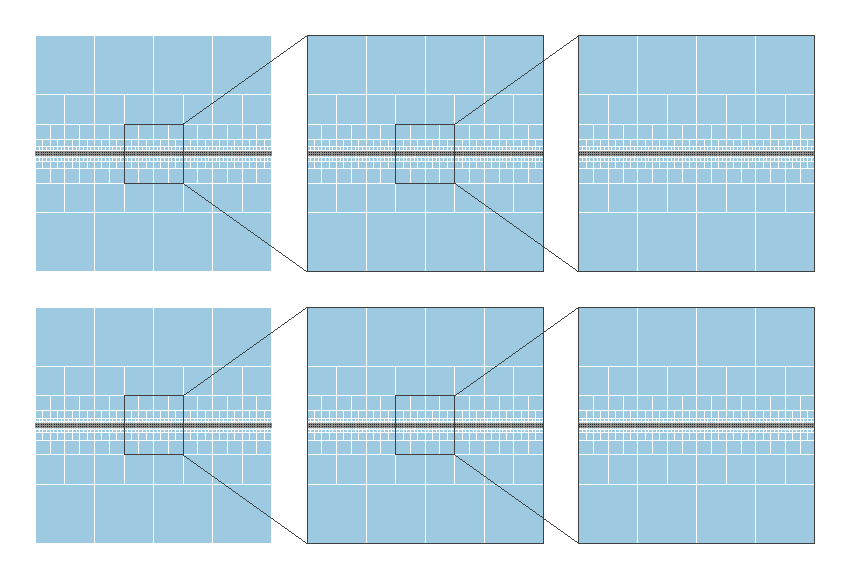
\includegraphics[width=\linewidth]{figures/global-refinement}
\caption{Subdivision with the Domain and Global components alone, near aligned configurations with ordinary viewing directions. Top: the plane $t=1/10$, $r_1=r_2=0$ around $s=1/4$, $r_3=0$ ($s$ horizontally, $r_3$ vertically). Bottom: the plane $s=1/5$, $r_2=r_3=0$ around $t=1/8$, $r_1=0$ ($t$ horizontally, $r_1$ vertically). From left to right, windows of half-width $1/8$, $1/32$ and $1/128$, each halved $14$ times; \fc{Global}{light blue pieces are eliminated by the Global component}, black pieces are unresolved. At every magnification a band of unresolved pieces remains along the aligned configurations: refinement alone never reaches a touch configuration.}
\label{fig:global-refinement}
\end{figure}
